%%
%% KCGS journal latex format example.
%% There are several options in this file, 
%% PLEASE READ THE FOLLOWING LINES BEFORE YOU USE.
%% 1. If you use KC2007 instead of MikTeX, use ``kotex'' package.
%% 2. If you don't have ``ifpdf'' package, 
%%    then use ``epsfig'' and ``epstopdf'' packages.
%%    (But usually you should have ``ifpdf'' package, 
%%    because the package is used in siggraph class.
%% 3. If you don't have ``caption'' package, 
%%    comment out "\usepackage[labelfont=bf]{caption}" command.
%% 4. There are several commands for squeezing figures and tables into a page.
%%    Uncomment those commands if you want to use them.
%% This file is tested under KC2008 and MikTex 2.4~2.5 with HLaTeX.
%%
%% If you have problems in using LaTeX, visit http://www.ktug.or.kr
%%
%% - 1st version 2007/08/22 Hyunjun Lee.
%% - 2nd version 2009/03/11 Hyunjun Lee.
%%   email: crowlove@postech.ac.kr
%%   Please do not email me if you have any questions or problems :)
%%

\documentclass[a4paper,twocolumn]{article}

%---------------------------------------------------------------------------
%% If you don't really know latex commands and changes you want to make,
%% you don't need to change anything up to "document begins" below.

\usepackage[hangul]{kotex}
\usepackage{dhucs-cmap}

%% Geometry package for page layout.
\usepackage{geometry}
\geometry{width=190mm, height=247mm, hmargin={1cm, 1cm}, vmargin={3cm, 2cm}}

%% We use one-half spacing.
\usepackage{setspace}
\onehalfspacing

%% Package to use both korean and english titles, authors, abstracts.
\usepackage{kcgs_utf}

%% The 'helvet' and 'times' packages define the typefaces used for
%% serif and sans serif type in this document. Computer Modern Roman 
%% is used for mathematics typesetting. The scale factor is set to .92
%% to bring the sans-serif type in line with the serif type.
\usepackage[scaled=.92]{helvet}
\usepackage{times}

%% The 'graphicx' package allows for the inclusion of EPS figures.
\usepackage{ifpdf}
	\ifpdf % compile with pdflatex
		\usepackage[pdftex]{graphicx}
	\else % latex => compile with dvipdfmx
		\usepackage{graphicx}
			\DeclareGraphicsExtensions{.jpg,.pdf,.png,.eps}
			\DeclareGraphicsRule{.jpg}{eps}{.bb}{}
			\DeclareGraphicsRule{.pdf}{eps}{.bb}{}
			\DeclareGraphicsRule{.png}{eps}{.bb}{}
	\fi

%% Or, if you don't have ``ifpdf'' package, use this two packages instead.
%\usepackage{epsfig}
%\usepackage{epstopdf}

%% Remove '제','절' from section names.
\kscntformat{section}{}{.}

%% Optional: the 'caption' package provides a nicer-looking replacement
%% for the standard caption environment. With 'labelfont=bf,'textfont=it',
%% caption labels are bold and caption text is italic.
%% You don't have to use this package if the package does not exist.
%\usepackage[labelfont=bf]{caption}

%% Uncomment following lines if you want to squeeze figures and tables into a page.
%\renewcommand{\topfraction}{0.95}
%\setcounter{bottomnumber}{1}
%\renewcommand{\bottomfraction}{0.95}
%\setcounter{totalnumber}{3}
%\renewcommand{\textfraction}{0.05}
%\renewcommand{\floatpagefraction}{0.95}
%\setcounter{dbltopnumber}{2}
%\renewcommand{\dbltopfraction}{0.95}
%\renewcommand{\dblfloatpagefraction}{0.95}

%---------------------------------------------------------------------------
% document begins

\begin{document}

%% Title.
\title{Sparse Ellipsometry: Portable Acquisition of Polarimetric SVBRDF	and Shape with Unstructured Flash Photography}

%% Author names.
\author{황인승$^{1\circ}$
\and 전석준$^{1}$
\and Adolfo Muñoz$^{3}$
\and Diego Gutierrez$^{3}$
\and Xin Tong$^{2}$
\and 김민혁$^{1*}$}

\affiliation{$^{1}$KAIST 
	\hspace{5mm} $^{2}$Microsoft Research Asia 
	\hspace{5mm} $^{3}$Universidad de Zaragoza - I3A}

\authoremail{
	$^{1}$\{ishwang, sjjeon, minhkim\}@vclab.kaist.ac.kr \hspace{5mm}
	$^{2}$xtong@microsoft.com \hspace{5mm}
	$^{3}$\{adolfo, didgog\}@unizar.es}

%% English title.
\entitle{Sparse Ellipsometry: Portable Acquisition of Polarimetric SVBRDF	and Shape with Unstructured Flash Photography}

%% English author names.
\enauthor{Inseung Hwang$^{1\circ}$
	\and Daniel S. Jeon$^{1}$
	\and Adolfo Muñoz$^{3}$
	\and Diego Gutierrez$^{3}$
	\and Xin Tong$^{2}$
	\and Min H. Kim$^{1*}$}

\enaffiliation{$^{1}$KAIST 
	\hspace{5mm} $^{2}$Microsoft Research Asia 
	\hspace{5mm} $^{3}$Universidad de Zaragoza - I3A}

% (Optional) Teaser
\teaser{
  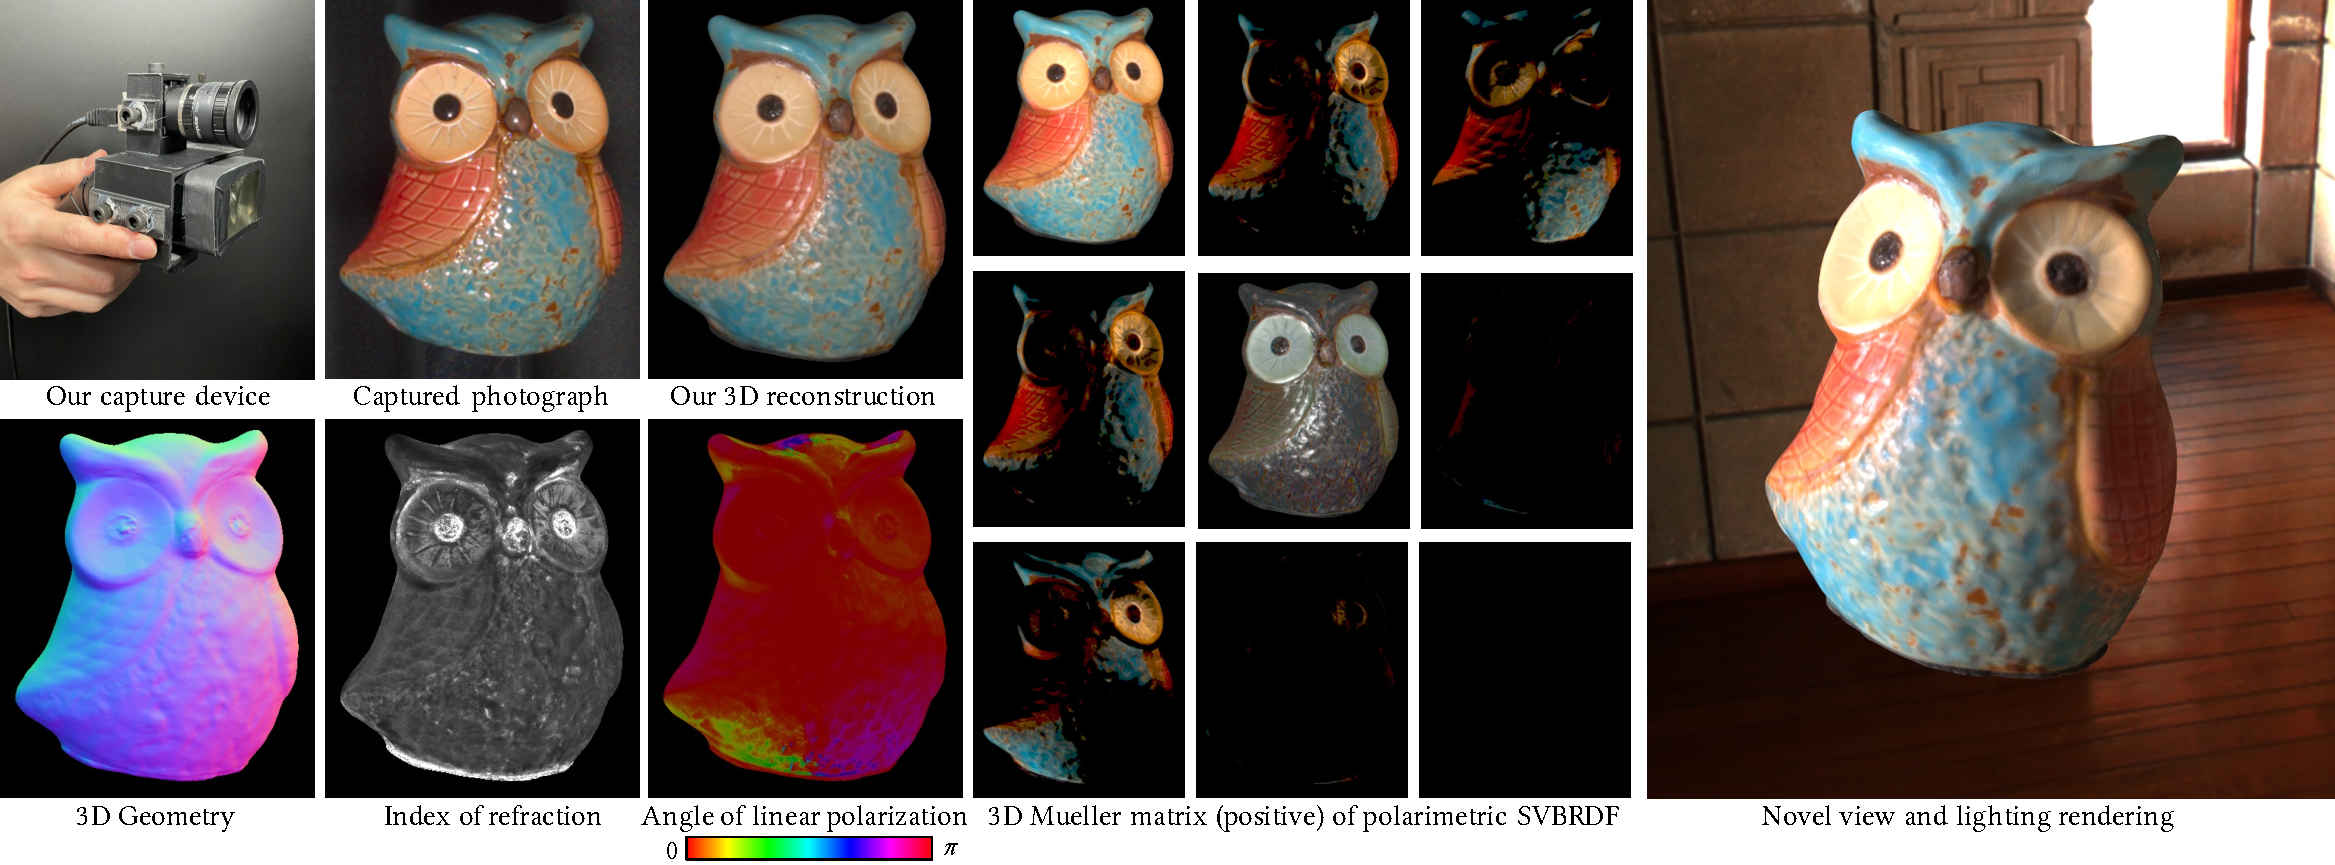
\includegraphics[width=0.95\textwidth]{fig/teaser.pdf}
  \caption{Teaser image. (10pt)}
  \label{fig:teaser}
}

%% Abstract.
\begin{abstract}
편광해석법(Ellipsometry)을 사용하면 물질의 편광 정보를 측정할 수 있으나 다양한 구성의 조명과 센서로 구성된 광학 부품의 정밀한 회전을 요구한다. 이로 인해 실험실 조건에서 정밀하게 캘리브레이션된 복잡한 촬영 장치에서 생성되며 일반적으로 오브젝트당 며칠 정도의 매우 긴 촬영 시간이 소요된다. 
%최근의 기술을 사용하면 편광의 공간적으로 변화하는(spatially-varying) 반사율 정보를 촬영할 수 있지만 단일 시점으로 제한되거나 모든 시점을 촬영할 수 있지만 오브젝트가 단일 균질 물질로 만들어진 구형 물체로 제한된다. 
본 연구는 편광 SVBRDF와 3D 형상을 동시에 촬영하는 휴대용 편광 획득 방법인 Sparse ellipsometry를 소개한다. 
%우리의 휴대용 장치는 기성품의 고정 광학 부품으로 구성되어 있다. 총 촬영 시간은 며칠이 아닌 개체당 20분에서 30분 사이이다. 
우리는 확산 및 반사 구성 요소와 단일 산란을 포함하는 완전한 편광 SVBRDF 모델을 개발하고 생성 모델링을 통한 반사 샘플의 데이터 증강을 사용하여 새로운 편광 인버스 렌더링(inverse rendering) 알고리즘을 고안한다. 우리의 결과는 실제 객체의 캡처된 편광 BRDF의 최근 실측 데이터셋과 일치함을 보여준다.

\end{abstract}

%% English abstract.
%\begin{enabstract}
%
%The ``Abstract'' title should be written in (bold, 14pt) font size and contents should be written in (10pt).
%Please write abstract of the paper.
%
%\end{enabstract}

%% Keywords that describe your work.
\keywords{편광 모습, 3D 재건, 물질 모습, 형상}
\enkeywords{Polarimetric appearance, 3D reconstruction,	material appearance, shape}

%% The ``\maketitle'' command should be excuted after abstract section and keywords are written.
\maketitle

%---------------------------------------------------------------------------
% paper begins

\section{서론}
\label{sec:introduction}
실제 객체의 BRDF(양방향 반사율 분포 함수)의 사실적인 모델링은 물리 기반 렌더링의 핵심 기술이다.
그러나 빛의 편광 상태에 대한 산란 효과는 인간의 눈으로 대부분의 경우 감지할 수 없기 때문에 일반적으로 무시되었다.
그러나 편광은 광학 센서로 쉽게 촬영할 수 있으며 물체의 기하 및 물질 속성에 대한 유용한 정보를 제공한다.

%편광해석법은 광학 측정을 사용하여 물질과의 상호 작용이 입사광의 편광 상태를 변경하는 방식을 특정한다~\cite{azzam2016stokes}. 
%최근의 이미지 기반 편광해석법에는 두 가지 주요 접근 방식이 있다. 실제 물체의 편광 SVBRDF를 캡처할 수 있지만 단일 시점으로 제한되는 방식과~\cite{Baek2018} 편광 정보를 모든 시야 방향에서 측정할 수 있지만 하나의 균질한 단일 물질로 구성된 구형 물체로 제한되는 방식이 있다~\cite{Baek2020}. 
최근의 기술을 사용하면 편광의 공간적으로 변화하는(spatially-varying) 반사율 정보를 촬영할 수 있지만 단일 시점으로 제한되거나 모든 시점을 촬영할 수 있지만 오브젝트가 단일 균질 물질로 만들어진 구형 물체로 제한된다.
또한 며칠 정도의 긴 촬영시간을 요구하며 정교한 광학 테이블 구성과 회전하는 광학 장비가 필요하다.
본 연구는 임의의 기하구조뿐만 아니라 모든 시점 방향에서 공간적으로 변하는 편광 물체를 동시에 촬영할 수 있는 최초의 연구이다. 기성품의 편광 카메라와 회전 요소가 필요 없는 선형 편광판이 달린 플래시라이트를 결합한 휴대용 장치를 이용한다. 
실제 데이터와 정확하게 일치하는 결과물을 내며 촬영 시간은 기존 접근 방식과 같이 며칠이 아닌 20분에서 30분 사이에 불과하다.

구조화되지 않은 희박하게 촬영된 이미지 세트에서 인버스 렌더링을 포함하는 최적화 알고리즘을 사용하여 편광 반사율과 3D 모양을 복원한다. 
난반사 및 정반사뿐만 아니라 단일 산란도 포함된 새로운 편광 SVBRDF 모델을 제안하며, 최근 연구의 실제 데이터셋을 통해 일치함을 확인한다.
매우 좁은 정반사 로브의 경우 정반사 파라미터를 추정하기 충분하지 않기 때문에, 새로운 합성 시점으로 입력을 증강하는 생성 모델링 전략을 고안한다.

\section{논문 작성 요령}
\label{sec:paper_writing_technique}


\subsection{논문 페이지 수 (굵게, 12pt)}
\label{subsec:paper_page_num}

10 페이지 이내.


\subsection{용지 및 여백처리}
\label{subsec:paper_and_margin}

용지: A4, 가로쓰기. \\
여백: 위쪽 30mm, 아래쪽 20mm, 왼쪽 10mm, 오른쪽 10mm.


\subsection{글꼴 및 크기}
\label{subsec:paper_font}

한글의 글꼴은 \{serif: 바탕, sans-serif: 고딕\}을 사용하며, 
영문은 \{serif: Times New Roman, sans-serif: Helvetica\}를 사용한다. 
본문의 내용은 기본적으로 serif 글꼴을 이용하여 작성한다.
글꼴의 크기는 각각의 내용 뒤의 괄호 안에 명시된 바와 같다.

본문의 줄 간격은 한글에서는 150\%, 워드에서는 1줄로 사용한다.


\subsection{연구방법}
\label{subsec:methods}

아래 순서대로 작성하며, 1$\sim$8항목은 1단 (column), 
9$\sim$11 항목은 2단으로 구성한다.

\begin{enumerate}
	\item 제목 (국문)
	\item 저자명 (국문), 발표자는 공동저자와 구분 처리한다 (예) 홍길동$^{\circ}$).
	\item 소속 (국문)
	\item 저자 e-mail address
	\item 제목 (영문)
	\item 저자명(국문), 발표자와 교신저자는 공동저자와 구분 처리한다. (예) 발표자: 홍길동$^{\circ}$, 교신저자: 홍길동$^{*}$)
	\item 소속 (영문)
	\item 요약
	\item 본문
	\begin{itemize}
		\item[-] 장 및 절에 해당되는 번호는 아라비아 숫자로 각각 1., 1.1 등과 같이 표기한다.
		\item[-] 그림의 명칭은 하단에, 표는 상단에 각각 Figure 1 및 Table 1로 표기하고 내용 또한 영문으로 작성한다.
	\end{itemize}
	\item 참고문헌
	\begin{itemize}
		\item[-] 본문 중에 참고문헌 번호를 쓰고, 그 문헌을 참고문헌란에 인용한 순서대로 기술한다.
		\item[-] 기술 순서는 아래의 예와 같이 저자, 제목, 학술지명, 권, 호, 쪽수 발행년도 순으로 작성한다.
	\end{itemize}
	\item 부록 (해당사항이 있는 경우만 작성한다.)
\end{enumerate}


\section{기타}
\label{sec:misc}

논문 작성 시 \ref{sec:paper_writing_technique}절에 명시된 요령을 지켜 주시기 바랍니다.


\section*{감사의 글}

감사의 글은 논문의 끝에 번호 없이 작성한다.

%---------------------------------------------------------------------------
% references

\bibliographystyle{IEEEtran}
\nocite{*}
\bibliography{ref}

%---------------------------------------------------------------------------
% done

\end{document}
